Несмотря на большую площадь Канады, многие её районы до сих пор не обжиты, и большая часть населения живёт вблизи южной границы. Трансканадская магистраль, построенная в 1962 году, соединяет людей вдоль этой полоски земли от Сент-Джона на востоке до Виктории на западе. Общая её протяжённость~--- 7821 км.

Канадцы любят хоккей. После хоккейного матча тысячи фанатов садятся в свои машины и едут домой от места проведения матча, что вызывает огромные пробки на дорогах. Один богатый инвестор хочет купить хоккейную команду и построить новый хоккейный стадион. Ваша задача --- помочь ему выбрать местонахождение стадиона, которое бы минимизировало пробки на дорогах после матча.

Страна состоит из городов, соединённых дорогами. Все дороги двусторонние, и между любыми двумя городами существует ровно один маршрут. Маршрут, соединяющий города $c_0$ и $c_k$ --- это последовательность различных городов $c_0, \cdots, c_k$ такая, что существует дорога из $c_{i-1}$ в $c_i$ для всех $i$. Новый стадион должен быть построен в одном из городов, назовём его городом со стадионом. После хоккейного матча, все фанаты, кроме тех, что живут в городе со стадионом, едут из города со стадионом в свой родной город. Величина пробки на каждой дороге пропорциональна количеству фанатов, которые проедут по этой дороге. Вам необходимо выбрать такое местонахождение стадиона, чтобы величина пробки на дороге с самой большой пробкой была минимально возможной. Если существуют несколько городов, одинаково подходящих для расположения стадиона, вы можете выбирать любой из них.

\begin{tabular}{ccc}
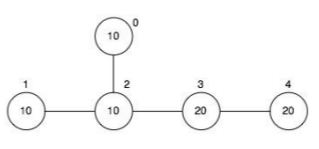
\includegraphics[scale=0.45]{traffic1.png} &
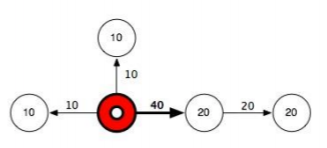
\includegraphics[scale=0.45]{traffic2.png} &
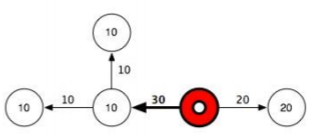
\includegraphics[scale=0.45]{traffic3.png}
\end{tabular}

Вам необходимо реализовать процедуру \t{LocateCentre(N,P,S,D)}, где $N$~--- положительное целое число, задающее количество городов. Города пронумерованы от $0$ до $N-1$. $P$~--- это массив из $N$ положительных целых чисел. Для каждого $i$ элемент массива $P[i]$~--- это количество фанатов, которые живут в городе с номером $i$. Общее количество фанатов, живущих во всех городах, будет не более $2\,000\,000\,000$. $S$ и $D$~--- это массивы из $N-1$ целых чисел каждый, которые задают местоположение дорог. Для каждого $i$ существует дорога, соединяющая два города с номерами $S[i]$ и $D[i]$. Процедура должна возвращать целое число~--- номер города, в котором необходимо построить стадион

Для примера рассмотрим дорожную сеть из пяти городов на левом из рисунков сверху. На этом рисунке в городах с номерами $0$, $1$ и $2$ живут по $10$ фанатов, а в городах с номерами $3$ и $4$ живут по $20$ фанатов. Средний рисунок показывает величину пробок, если стадион будет построен в городе с номером $2$. В этом случае наибольшая пробка величиной $40$ будет достигаться на дороге, обозначенной жирной стрелкой. Правый рисунок показывает величину пробок, если стадион будет построен в городе с номером $3$. В этом случае наибольшая пробка величиной $30$ будет достигаться на дороге, обозначенной жирной стрелкой. Таким образом, город с номером $3$ лучше подходит для строительства стадиона, чем город с номером $2$. Это 3-й тестовый пример